
% Этот шаблон документа разработан в 2014 году
% Данилом Фёдоровых (danil@fedorovykh.ru) 
% для использования в курсе 
% <<Документы и презентации в \LaTeX>>, записанном НИУ ВШЭ
% для Coursera.org: http://coursera.org/course/latex .
% Исходная версия шаблона --- 
% https://www.writelatex.com/coursera/latex/5.1

\documentclass[c]{beamer}  % [t], [c], или [b] --- вертикальное выравнивание на слайдах (верх, центр, низ)
%\documentclass[handout]{beamer} % Раздаточный материал (на слайдах всё сразу)
%\documentclass[aspectratio=169]{beamer} % Соотношение сторон

%\usetheme{Berkeley} % Тема оформления
%\usetheme{Bergen}
\usetheme{EastLansing}
%\usetheme{AnnArbor}
\usecolortheme{seahorse} % Цветовая схема

%\useinnertheme[shadow=true]{rounded}
\usepackage{etoolbox}
\definecolor{mygreen}{cmyk}{0.4, 0, 0.6, 0}
\definecolor{mygreen2}{cmyk}{0.8324,0,1,0.298}
\setbeamercolor{block body}{bg=blue!5!white}
\setbeamercolor{block title}{bg=blue!20!white}

\setbeamercolor{block body alerted}{bg=red!5!white!}
\setbeamercolor{block title alerted}{bg=red!20!white!}

%\begin{comment}
%\newenvironment<>{plus}[1]{%
%	\setbeamercolor{block body}{bg=green!5!white!}
%	\setbeamercolor{block title}{fg=mygreen2,bg=mygreen!50!white!}
%	\begin{block}#2{#1}}{\end{block}}
%\end{comment}

\setbeamertemplate{itemize items}[circle]

%\setbeamercolor{structure}{bg=green!20!yellow}
%\useinnertheme{circles}
%\useinnertheme{rectangles}


%%% Работа с русским языком
\usepackage{cmap}					% поиск в PDF
\usepackage{mathtext} 				% русские буквы в формулах
\usepackage[T2A]{fontenc}			% кодировка
\usepackage[utf8]{inputenc}			% кодировка исходного текста
\usepackage{subfigure} 				% 2 картинки в одном ряду
%\usepackage[english,russian]{babel}	% локализация и переносы

%% Beamer по-русски
\newtheorem{rtheorem}{Теорема}
\newtheorem{rproof}{Доказательство}
\newtheorem{rexample}{Пример}

\newtheorem{proposition}{Proposition}

%%% Дополнительная работа с математикой
\usepackage{amsmath,amsfonts,amssymb,amsthm,mathtools} % AMS
\usepackage{icomma} % "Умная" запятая: $0,2$ --- число, $0, 2$ --- перечисление

%% Номера формул
%\mathtoolsset{showonlyrefs=true} % Показывать номера только у тех формул, на которые есть \eqref{} в тексте.
%\usepackage{leqno} % Нумерация формул слева

%% Свои команды
\DeclareMathOperator{\sgn}{\mathop{sgn}}

%% Перенос знаков в формулах (по Львовскому)
\newcommand*{\hm}[1]{#1\nobreak\discretionary{}
	{\hbox{$\mathsurround=0pt #1$}}{}}

%%% Работа с картинками
\usepackage{graphicx}  % Для вставки рисунков
%\graphicspath{{LaTex/}{images/}}  % папки с картинками
\setlength\fboxsep{3pt} % Отступ рамки \fbox{} от рисунка
\setlength\fboxrule{1pt} % Толщина линий рамки \fbox{}
\usepackage{wrapfig} % Обтекание рисунков текстом

%%% Работа с таблицами
\usepackage{array,tabularx,tabulary,booktabs} % Дополнительная работа с таблицами
\usepackage{longtable}  % Длинные таблицы
\usepackage{multirow} % Слияние строк в таблице

%%% Программирование
\usepackage{etoolbox} % логические операторы

%%% Другие пакеты
\usepackage{lastpage} % Узнать, сколько всего страниц в документе.
\usepackage{soul} % Модификаторы начертания
\usepackage{csquotes} % Еще инструменты для ссылок
%\usepackage[style=authoryear,maxcitenames=2,backend=biber,sorting=nty]{biblatex}
\usepackage{multicol} % Несколько колонок

%%% Картинки
\usepackage{tikz} % Работа с графикой
\usepackage{pgfplots}
\usepackage{pgfplotstable}

%References
\usepackage[natbibapa]{apacite}
\usepackage{bibentry}

\title[Thesis]{Attitudes towards ethnic diversity and provision of public goods}
\author[Dedyukhin Ivan]{Dedyukhin Ivan\thanks{Advisor: Shlomo Weber}}
\date{\today}
\institute[NES]{New Economic School}

\begin{document}
	
	\frame[plain]{\titlepage}	% Титульный слайд

    \section{Introduction}

    \begin{frame}{Introduction}
        \begin{itemize}
            \item Ethnic diversity is a determinant of economic performance (\cite{Russia}, \cite{Africa})
            \pause
            \item Ethnic diversity is a determinant of public good provision (\cite{AlesinaDivision}, \cite{Kenya}, \cite{Indonesia}, \cite{transfer})
            \pause
            \item There is no consensus about mechanism (\cite{WhyUndermine}, \cite{Cooperation}, \cite{difference})
            \pause
            \item The attitude towards ethnic diversity matters (\cite{Refuges})
            \pause
            \item \textbf{Does attitude towards ethnic diversity influence public good provision?}
        \end{itemize}
    \end{frame}
    
    \section{Model}
    
    \begin{frame}{Model setup}
        \begin{itemize}
            \item Utility $u(x(I), g(I), H(I) )$
            \begin{enumerate}
                \item private consumption ($x$) of agent in group $I$
                \item public goods consumption ($g$) of agent in group $I$
                \item ethnic heterogeneity ($H$) of agent in group $I$
                \pause
                \begin{itemize}
                    \item ethnic heterogeneity reduces the utility an agent derives from consuming the public good $g$
                    \item \textbf{Consumption of public good requires interaction with other ethnicities}
                    \item Determinants of heterogeneity are fractionalization and attitude
                \end{itemize}
            \end{enumerate}
            \pause
            \item $U = x + \gamma((1 - H) g)^\beta $
            \pause
            \item First best provision is
            \[ g^{FB} = \left( \gamma\beta \sum_{I} p(I) (1-H(I))^{\beta} \right) ^\frac{1}{1 - \beta }  \]
        \end{itemize}
    \end{frame}
    
    \begin{frame}{Private provision}
        \begin{itemize}
            \item Suppose that public goods are financed through private provision
            \item Budget constraint is
            \[ x(I) + g_i(I) \le w(I) \]
            \item Utility is
            \[ U = w_i(I) - g_i(I) + \gamma( (1 - H(I) ) g)^\beta \] 
            \pause
            \item Equilibrium is
            \[ g^{PP} = (\beta\gamma  ( 1 - \min_{I} H(I)))^\frac{\beta}{1 -\beta} \]
            \pause
            \begin{proposition}
            Worse attitude (higher heteregoneity) means lower amount of public good if it is provided voluntary 
            \end{proposition}
        \end{itemize}
    \end{frame}
    
    \begin{frame}[allowframebreaks]{State provision}
        \begin{itemize}
            \item Suppose that public goods are financed from taxes by benevolent government
            \item Government maximization problem is 
            \[ \max_{t\in[0,1], g\ge 0} \sum_{I} p(I) ( (1-t)w_i(I) + \gamma( (1 - H(I)) g)^\beta)  \]
            \[\text{s.t. } g \le t\sum_{I} p(I) w_i(I)  \]
            \pause
            \item Equilibrium is
            \[ g^{SP} = \min \left\{ \left( \gamma  \beta\sum_{I} p(I) (1 - H(I))^\beta \right)^\frac{1}{1 - \beta}; W \right\} \]
            \pause
            \begin{proposition}
            Worse attitude (higher heteregoneity) means lower amount of public good if it is provided by state 
            \end{proposition}
        \end{itemize}
    \end{frame}
    
    \section{Data}
    
    \begin{frame}{Data sources}
        \begin{itemize}
            \item 97 U.S. cities for the period 2006 - 2017
            \pause
            \item Individual data from \hyperlink{https://usa.ipums.org/usa/}{IPUMS USA} project
            \begin{itemize}
                \item FRAC measures the probability that two randomly drawn people from a city belong to different ethnic groups
                \pause
                \item The attitude towards diversity index (INDEX)
                \begin{itemize}
                    \item \textbf{the share of co-racial marriages in a city's total number of marriages}
                \end{itemize}
            \end{itemize}
            \pause
        \item The Fiscally Standardized Cities (FiSC) database from Lincoln Institute of Land Policy
        \begin{itemize}
            \item This database makes it possible to compare cities' finances
            \item Fiscal variables are calculated per capita in 2017 USD.
            \item Dependent variables are share of total spending by aim
        \end{itemize}
        \end{itemize}
    \end{frame}
    
    \begin{frame}{Descriptive statistics}
        \begin{table}[h!]
        \tiny
        \centering
        {
\def\sym#1{\ifmmode^{#1}\else\(^{#1}\)\fi}
\begin{tabular}{l*{1}{cccc}}
\hline\hline
                    &\multicolumn{4}{c}{(1)}                            \\
                    &\multicolumn{4}{c}{}                               \\
                    &        Mean&          S.D.&         Min&         Max\\
\hline
City Population     &    557022.8&     1060585&       80215&     8475976\\
Log of city population&    12.68124&    .8683314&    11.29247&    15.95275\\
Taxes collected     &    2198.987&    1221.208&      732.71&    11223.87\\
General expenditures&    5952.036&    2291.052&     2033.46&    21446.74\\
Secondary education expenditures&    2007.007&    644.0921&      544.84&     4811.56\\
Libraries expenditures&    51.92246&    34.49064&           0&      585.74\\
Public welfare expenditures&    268.4206&    604.8267&           0&     5725.41\\
Hospital expenditures&    282.1485&     582.429&           0&     4432.26\\
Health expenditures &    217.3635&    228.5996&           0&     2198.96\\
Highways expenditures&    232.4785&    133.0477&        6.21&     1067.75\\
Public safety expenditures&    773.3932&    265.9719&      268.43&     2312.49\\
Sewerage expenditures&    245.4629&    160.8913&           0&     1070.79\\
Administration expenditures&    308.1253&    168.1048&       56.07&     1698.06\\
Parks and recreation expenditures&    178.9966&    136.8253&        1.03&     1410.71\\
Ethnic fractionalization&    .4420603&    .1377596&    .0853811&    .6934802\\
Ethnic fractionalization among married&    .4580479&    .1321692&    .0917879&    .6981086\\
Reynal-Querol polarization&    .6988702&    .1972032&     .140374&    .9807938\\
Alienation          &     .189907&    .0825309&    .0536585&    .4158192\\
Mean HH income      &    634356.8&    404314.1&    88548.67&     2851736\\
Inequality          &    11.32726&    7.060934&    1.225278&     47.1012\\
\hline
Observations        &         900&            &            &            \\
\hline\hline
\end{tabular}
}

        \caption{Descriptive statistic for US cities 2006 - 2017}
        \label{tab:desc}
    \end{table}
    \end{frame}
    
    \begin{frame}{Alienation and fractionalization}
    I have an alienation variation for fixed fractionalization
    \begin{figure}[h]
                \centering
                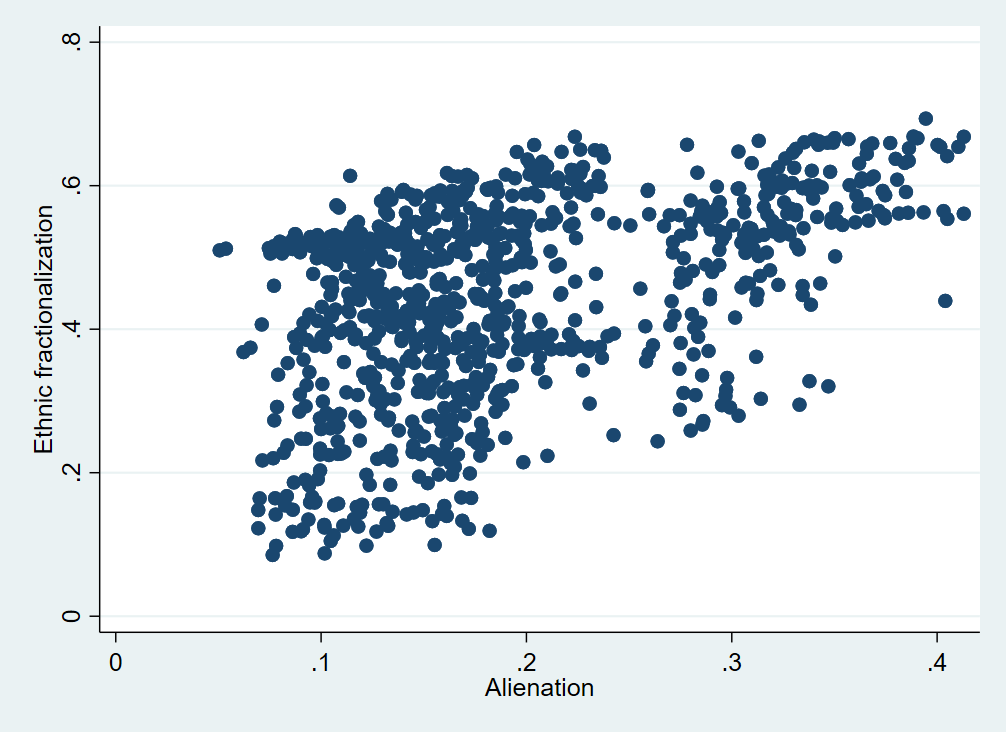
\includegraphics[scale = 0.2]{Thesis/Figures/frac-index.png}
                \caption{Scatter plot for attitude index and ethnic fractionalization}
                \label{fig:frac-index}
    \end{figure}
    \end{frame}
    
    \begin{frame}{Different fractionalizations}
    Total fractionalization and fractionalization among married are the same
    \begin{figure}[h]
        \centering
        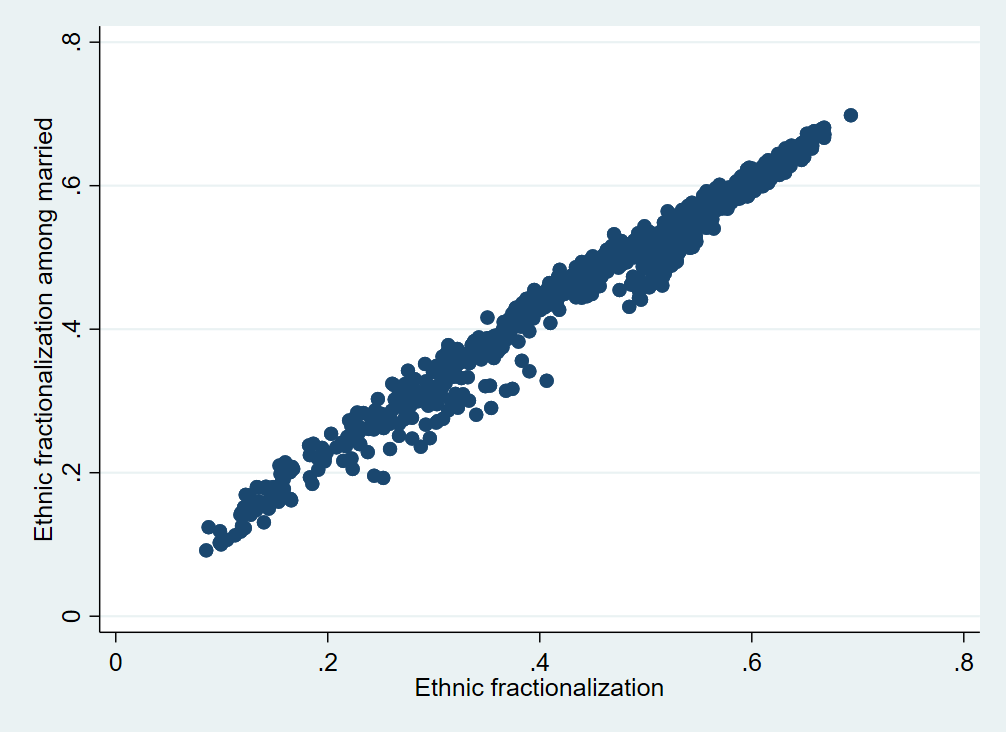
\includegraphics[scale = 0.2]{Thesis/Figures/frac-frac.png}
        \caption{Scatter plot for general fractionalization and fractionalization among married}
        \label{fig:frac-frac}
    \end{figure}
    \end{frame}
    
    \begin{frame}{Geographical variation}
    Lack of geographical variation for big cities
    \begin{figure}[h]
        \centering
        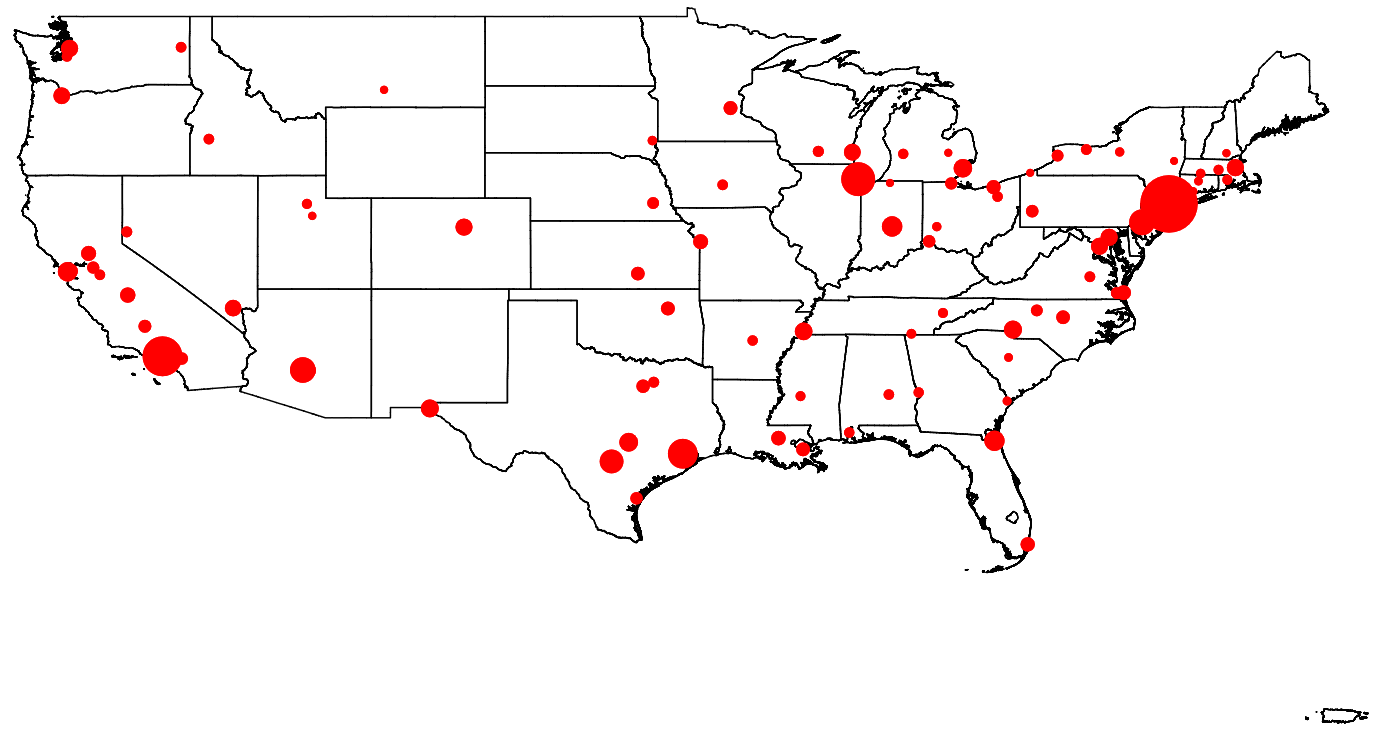
\includegraphics[scale = 0.2]{Thesis/Maps/city_population.png}
        \caption{The map of U.S. cities in dataset. The size of the points is proportional to the population.}
        \label{fig:frac-frac}
    \end{figure}
    \end{frame}
    
    \section{Empirics}

    \begin{frame}{Identification strategy}
        \begin{itemize}
            \item \textbf{I believe in exogeneity}
            \pause
            \item Possible multicollinearity 
            \pause
            \item Propensity-score-matching and dose-response function (\cite{prop}, \cite{package})
            \pause
            \item Generalized propensity score:
            \[ r(t, x)=f_{INDEX \mid X}(t \mid x) \]
            \[ GPS = r(INDEX, X) \]
            \pause
            \item Conditional expectation of the outcome
            \[ \beta(t, r)=E(Y \mid T=t, R=r) \]
            \[ Fiscal_{it} = \alpha + \beta_1 \times INDEX_{it} + \beta_2 \times GPS_{it} + \beta_3 \times INDEX_{it} \times GPS_{it} \]
            \pause
            \item Dose-response function:
            \[ \mu(t)=E[\beta\{t, r(t, X)\}] \]
        \end{itemize}
    \end{frame}
    
    \begin{frame}{Results}
    \noindent

    \end{frame}
    
    \begin{frame}{Results}
        \begin{figure}[h!]
        \centering
        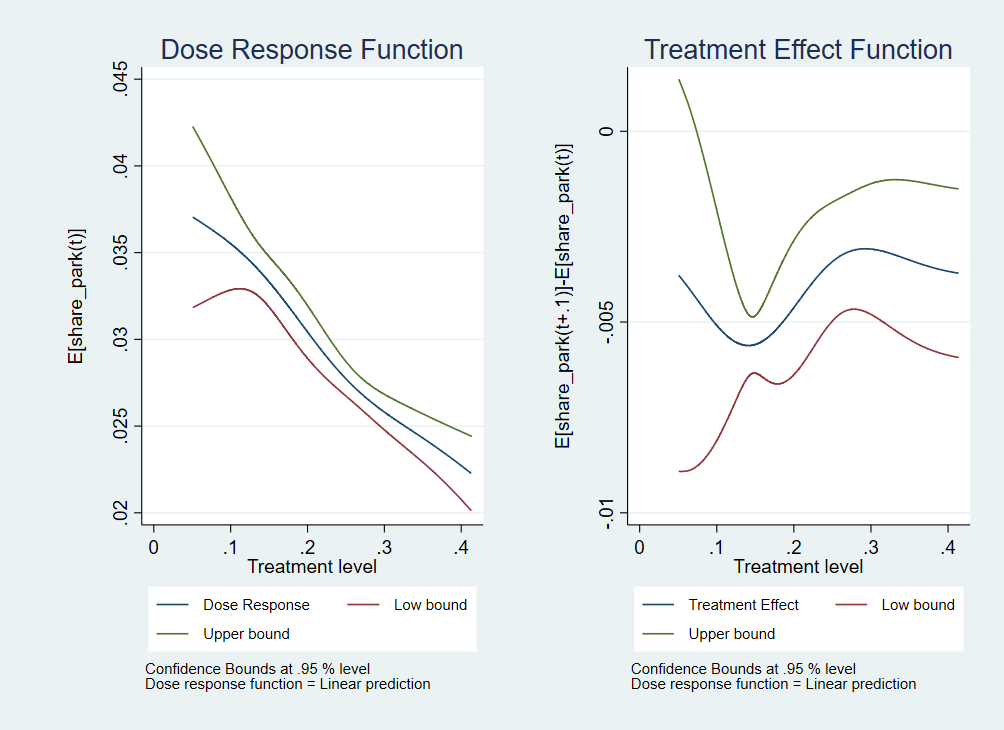
\includegraphics[scale = 0.25]{Thesis/Figures/graph_parks.png}
        \caption{Dose-response function (left) and its derivative (right) for parks and recreational spending}
        \label{fig:graph_educ}
    \end{figure}
    \end{frame}
    
    \begin{frame}{Results}
        \begin{figure}[h!]
        \centering
        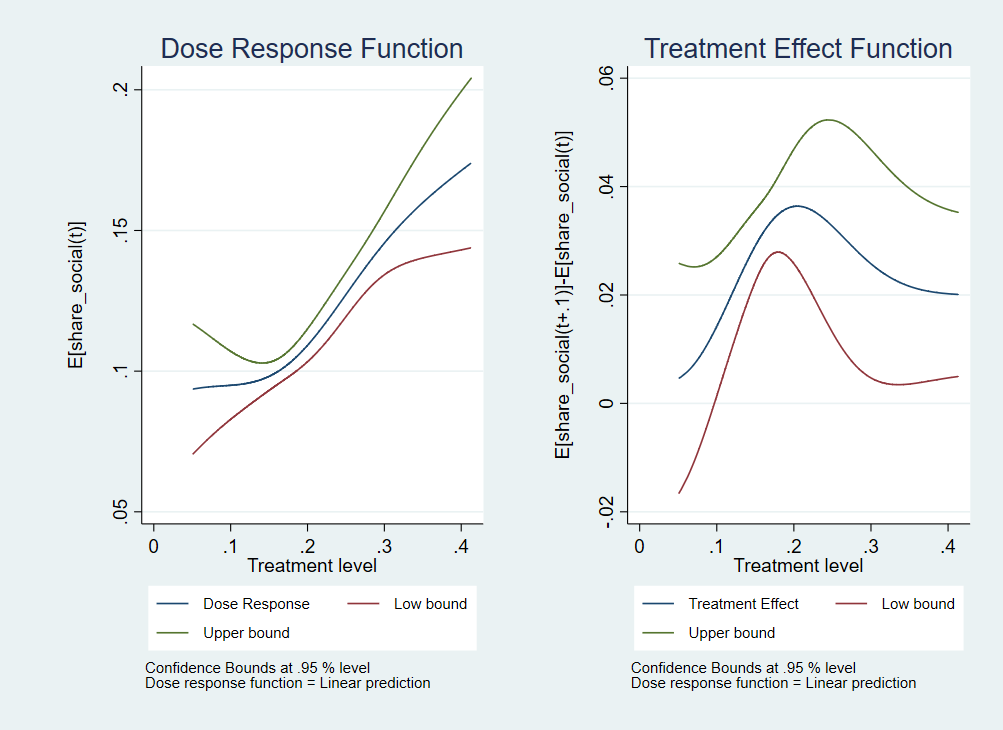
\includegraphics[scale = 0.25]{Thesis/Figures/graph_social.png}
        \caption{Dose-response function (left) and its derivative (right) for social spending}
        \label{fig:graph_educ}
    \end{figure}
    \end{frame}
    
    \section{Conclusion}
    
    \begin{frame}{Conclusion}
        \begin{itemize}
            \item I have found that worse attitude towards ethnic diversity decrease provision of parks and recreational facilities and secondary education
            \begin{itemize}
                \item This public goods are based in interaction of people
            \end{itemize}
            \pause
            \item I have found that worse attitude towards ethnic diversity increase welfare and social services spending
            \begin{itemize}
                \item Worse attitude may cause lower economic performance and greater criminality
                \item More people needs help
            \end{itemize}
            \pause
            \item Possible drawbacks of the paper:
            \begin{itemize}
                \item Lack of geographical variation
                \item Lack of observations
                \item Different levels have different incentives
                \item Inappropriate proxy for Alienation
            \end{itemize}
            \item Further research is required
        \end{itemize}
    \end{frame}
    
    
    \begin{frame}[allowframebreaks]{References}
        \bibliographystyle{apacite}
        \bibliography{ref}
    \end{frame}
    

\end{document}
